\documentclass[letterpaper,fleqn]{article}
\usepackage[spanish,es-noshorthands]{babel}
\usepackage[utf8]{inputenc} 
\usepackage[left=1cm, right=1cm, top=1.5cm, bottom=1.7cm]{geometry}
\usepackage{mathexam}
\usepackage{amsmath}
\usepackage{graphicx}
\usepackage{tikz,pgf}

\ExamClass{
\includegraphics[height=16pt]{Images/logo-sed.png} Matemáticas $6^{\circ}$}
\ExamName{Nivelación 2014}
\ExamHead{
\includegraphics[height=16pt]{Images/logo-colegio.png} IEDAB}
\newcommand{\LineaNombre}{%
\par
\vspace{\baselineskip}
Nombre:\hrulefill \; Curso: \underline{\hspace*{48pt}} \; Fecha: \underline{\hspace*{2.5cm}} \relax
\par}
\let\ds\displaystyle

\begin{document}
\ExamInstrBox{
Respuesta sin justificar mediante procedimiento no será tenida en cuenta en la calificación. Escriba sus respuestas en el espacio indicado. Tiene 60 minutos para contestar esta prueba.}
\LineaNombre
\begin{enumerate}
 \item Realice las siguientes operaciones:
 \begin{enumerate}
 \item $3+6\cdot 5-3\cdot 4-2=$\noanswer[20pt]
 \item $7\cdot 3+[6+2\cdot (8\div 4+3\cdot 2)-7\cdot 2]+9\div 3=$\noanswer[20pt]
 \end{enumerate}
 \item Resuelva los siguientes problemas:
 \begin{enumerate}
 \item Don Tomás quiere repartir unos libros entre sus hijos. Puede hacerlo dándoles 1 al mayor, 2 al segundo, 3 al tercero \ldots Otro modo de repartirlos sería dar 7 a cada uno. ¿Cuántos hijos y cuántos libros tiene don Tomás?\noanswer
 \item Maité quiere comprar sellos. Tiene menos de 100 pesetas, si los compra todos de 5 pesetas, le sobra una peseta. Si los compra de 8 pesetas le sobran 6 pesetas. Le falta una peseta para comprar un n\'{u}mero exacto de sellos de 29 pesetas. ¿Cu\'{a}nto dinero tiene Mait\'{e}?\noanswer
 \end{enumerate}
 \item ¿Cuál es el menor número que tiene por divisores 3, 4 y 12?\noanswer[36pt]
 \item Compruebe que para saber si un número menor que 100 es primo, es suficiente con dividir por 2, 3, 5 y 7. ¿Por cuántos números como máximo tendrá que dividir para saber si es primo el número 497?\noanswer
 \item En una granja se ha recogido un número de huevos entre setecientos y ochocientos. Forman un número exacto de docenas. También se podrían colocar exactamente en cartones de 15 huevos. ¿Cuántos huevos se han recogido en la granja?\noanswer
   \newpage
\begin{minipage}{.6\textwidth}
\item Si se eliminan 3 de los doce primeros divisores de 216, se puede conseguir con los otros nueve, sin repetir ninguno el siguiente cuadrado mágico multiplicativo, de manera que el producto de los tres números que ocupan cualquiera de las filas, columnas o diagonales, es siempre 216.
\end{minipage} \hfill
\begin{minipage}{.35\textwidth}
\begin{tikzpicture}
\draw (0,0) grid (3,3);
\node at (1.5,.5){36};
\node at (1.5,1.5){6};
\end{tikzpicture}
\end{minipage}
\item En una clase de 24 alumnos, $\frac{5}{8}$ son chicos. ¿Cuántos chicos y chicas hay en clase?\noanswer[72pt]
\item Ordene de menor  mayor las fracciones:
\begin{enumerate}
\item $\dfrac{8}{7}$, $\dfrac{9}{8}$, $\dfrac{5}{4}$\noanswer[20pt]
\item $\dfrac{4}{5}$, $\dfrac{5}{6}$, $\dfrac{8}{10}$, $\dfrac{3}{4}$\noanswer[20pt]
\end{enumerate}
\item Realice las siguientes operaciones simplificando los resultados cuando se pueda
\begin{enumerate}
\item $\dfrac{3}{4}+\dfrac{5}{6}+\dfrac{6}{8}=$\noanswer[20pt]
\item $\dfrac{7}{8}+\dfrac{3}{6}-\dfrac{5}{12}=$\noanswer[20pt]
\end{enumerate}
\begin{minipage}{.45\textwidth}
\item El siguiente gr\'{a}fico expresa el n\'{u}mero de refrescos consumidos durante 6 meses en un bar de la capital
\end{minipage} \hfill
\begin{minipage}{.55\textwidth}
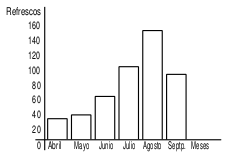
\includegraphics[scale=1]{Images/barras.png} 
\end{minipage}
\begin{enumerate}
\item ¿Cómo se denomina este tipo de gráfica?
\item ¿En qué mes se consumieron más refrescos?
\item ¿Durante que mes se consumieron menos refrescos?
\item Interprete la gráfica
\end{enumerate}
 \end{enumerate}
\end{document}
